\documentclass[11pt]{article}

\usepackage{mathtools}
\usepackage{mathrsfs}
\usepackage{amssymb}
\usepackage[latin1]{inputenc}
\usepackage[margin=0.5in]{geometry}
\usepackage{graphicx}
\usepackage{caption}
\usepackage{subcaption}
\usepackage{float}

\everymath{\displaystyle}
\setlength\parindent{0pt}

\begin{document}
\title{Stanford CS 229, Public Course, Problem Set 4}
\date{\today}
\author{Dylan Price}
\maketitle 

% custom commands
\newcommand{\xith}[0]{x^{(i)}}
\newcommand{\yith}[0]{y^{(i)}}
\newcommand{\zith}[0]{z^{(i)}}
\newcommand{\sums}[0]{\sum_{s' \in \mathbb{S}}}

\section*{1}

\subsection*{a)}
Given training set $\{(x^{(1)},y^{(1)},z^{(1)}),...,(x^{(m)},y^{(m)},z^{(m)})\}$, write the log-likelihood of the parameters and derive the maximum likelihood estimate for $\phi$, $\theta_0$, and $\theta_1$. \\

First we write the likelihood for a single point $(\xith, \yith, \zith)$:\\
\begin{align*}
    \mathscr{L}(\xith,\yith,\zith) = g(\phi^T \xith)^{\zith} (1 - g(\phi^T \xith))^{1 - \zith} \frac{1}{\sqrt{2 \pi} \sigma} \exp{\frac{-(\yith - \theta_{\zith}^T \xith)^2}{2 \sigma^2}} \\ 
\end{align*}
Then the log-likelihood of the parameters is:
\begin{align*}
    \ell(\phi,\theta_{\zith}) &= \log \prod_{i=1}^m L(\xith,\yith,\zith) \\
                              &= \sum_{i=1}^m \log\big[g(\phi^T \xith)^{\zith} (1 - g(\phi^T \xith))^{1 - \zith}\big] + \log\big[\frac{1}{\sqrt{2 \pi} \sigma} \exp{\frac{-(\yith - \theta_{\zith}^T \xith)^2}{2 \sigma^2}}\big] \\
                              &= \sum_{i=1}^m \zith \log g(\phi^T \xith) + (1 - \zith) \log (1 - g(\phi^T \xith)) + \log\big[\frac{1}{\sqrt{2 \pi} \sigma} \exp{\frac{-(\yith - \theta_{\zith}^T \xith)^2}{2 \sigma^2}}\big] \\
                              &= \sum_{i=1}^m \zith \log g(\phi^T \xith) + (1 - \zith) \log (1 - g(\phi^T \xith)) + \log (\frac{1}{\sqrt{2 \pi} \sigma}) +  \frac{-(\yith - \theta_{\zith}^T \xith)^2}{2 \sigma^2} \\
                              &= \sum_{i=1}^m \zith \log g(\phi^T \xith) + (1 - \zith) \log (1 - g(\phi^T \xith)) + \log (\frac{1}{\sqrt{2 \pi} \sigma}) \\
                              &\quad\quad\quad - 1\{\zith = 0\} \frac{(\yith - \theta_0^T \xith)^2}{2 \sigma^2} - 1\{\zith = 1\} \frac{(\yith - \theta_1^T \xith)^2}{2 \sigma^2} \\
\end{align*}
Now take the gradient with respect to $\theta_0$ and set equal to $0$:
\begin{align*}
    \nabla_{\theta_0} \ell(\phi,\theta_0,\theta_1) &= \nabla_{\theta_0} \sum_{i=1}^m -1\{\zith = 0\} \frac{(\yith - \theta_0^T \xith)^2}{2 \sigma^2} \\ 
                                                   &= - \sum_{i=1}^m 1\{\zith = 0\} \frac{-2 \yith \xith + 2 \xith \theta_0^T \xith}{2 \sigma^2} \\
                                        \text{set} &= 0 \\
                                                 0 &= \sum_{i=1}^m 1\{\zith = 0\} (-\yith \xith + \xith \theta_0^T \xith) \\
    \sum_{i=1}^m 1\{\zith = 0\} \xith \theta_0^T \xith &= \sum_{i=1}^m 1\{\zith = 0\} \yith \xith \\
\end{align*}
Let $X_{z = 0}$ and $\vec{y}_{z=0}$ be equal to the design matrices except that all entries where $z = 1$ are $0$. Then the above is equivalent to:
\begin{align*}
    X_{z=0}^T X_{z=0} \theta_0 &= X_{z=0}^T \vec{y}_{z=0} \\
                      \theta_0 &= (X_{z=0}^T X_{z=0})^{-1} X_{z=0}^T \vec{y}_{z=0} \\
                      &\text{and similarly,} \\
                      \theta_1 &= (X_{z=1}^T X_{z=1})^{-1} X_{z=1}^T \vec{y}_{z=1} \\
\end{align*}
Now find the gradient and hessian of $\ell(\phi,\theta_0,\theta_1)$ with respect to $\phi$:
\begin{align*}
    \nabla_\phi \ell(\phi,\theta_0,\theta_1) &= \nabla_\phi \sum_{i=1}^m \zith \log g(\phi^T \xith) + (1 - \zith) \log (1 - g(\phi^T \xith)) \\
                                             &= \sum_{i=1}^m \frac{\zith}{g(\phi^T \xith)} \xith g(\phi^T \xith) (1 - g(\phi^T \xith)) + \frac{1 - \zith}{1 - g(\phi^T \xith)} -\xith g(\phi^T \xith)(1 - g(\phi^T \xith)) \\
                                             &= \sum_{i=1}^m \big[ \zith (1 - g(\phi^T \xith)) - (1 - \zith) g(\phi^T \xith) \big] \xith \\
                                             &= \sum_{i=1}^m \big[ \zith - \zith g(\phi^T \xith) - g(\phi^T \xith) + \zith g(\phi^T \xith) \big] \xith \\
                                             &= \sum_{i=1}^m \big[ \zith - g(\phi^T \xith) \big] \xith \\
  \nabla_\phi^2 \ell(\phi,\theta_0,\theta_1) &= \sum_{i=1}^m - g(\phi^T \xith)(1 - g(\phi^T \xith)) \xith {\xith}^T \\
\end{align*}

\subsection*{b)}
$\ell(\phi,\theta_0,\theta_1)$ is the same as part (a):
\begin{align*}
    \ell(\phi,\theta_0,\theta_1) = \sum_{i=1}^m \log p(\yith|\xith,\zith) p(\zith|\xith) \\
\end{align*}
\textbf{E-step}\\
We want $Q_i(\zith)$ to be proportional to $p(\yith|\xith,\zith) p(\zith|\xith)$ so that Jensen's inequality holds with equality. \\
Therefore let $Q_i(\zith) = p(\yith|\xith,\zith) p(\zith|\xith)$. During the E-step, we calculate $Q_i(\zith = 0)$ and $Q_i(\zith = 1)$ for all $i$, using the formulas given in the problem statement and our current estimate of the parameters.\\

\textbf{M-step}\\
$\phi,\theta_0,\theta_1 := \arg \max_{\phi,\theta_0,\theta_1} \sum_{i=1}^m \sum_{\zith=0}^{1} Q_i(\zith) \log \frac{p(\yith|\xith,\zith)p(\zith|\xith)}{Q_i(\zith)}$\\
Find the closed-form solution for $\theta_0$ by taking the gradient with respect to $\theta_0$ and setting equal to $0$.
\begin{align*}
    &\nabla_{\theta_0} \sum_{i=1}^m \sum_{\zith=0}^{1} Q_i(\zith) \log \frac{p(\yith|\xith,\zith;\theta_{\zith})p(\zith|\xith;\phi)}{Q_i(\zith)} \\
    &\text{Let $1\{\text{guess } \zith = 0\}$ be equivalent to $1\{Q_i(\zith = 0) > Q_i(\zith = 1)\}$} \\
    &= \nabla_{\theta_0} \sum_{i=1}^m 1\{\text{guess } \zith = 0\} Q_i(\zith = 0) \log \frac{p(\yith|\xith,\zith=0;\theta_0) p(\zith=0|\xith;\phi)}{Q_i(\zith=0)} \\
    &= \nabla_{\theta_0} \sum_{i=1}^m 1\{\text{guess } \zith = 0\} Q_i(\zith = 0) \big[ \log p(\yith|\xith,\zith=0;\theta_0) + \log p(\zith=0|\xith;\phi) - \log Q_i(\zith=0) \big] \\
    &= \nabla_{\theta_0} \sum_{i=1}^m 1\{\text{guess } \zith = 0\} Q_i(\zith=0) \log p(\yith|\xith,\zith=0;\theta_0) \\
    &= \nabla_{\theta_0} \sum_{i=1}^m 1\{\text{guess } \zith = 0\} Q_i(\zith=0) \log \big( \frac{1}{\sqrt{2 \pi} \sigma} \exp{\frac{-(\yith-\theta_0^T \xith)^2}{2 \sigma^2}}\big) \\
    &= \nabla_{\theta_0} \sum_{i=1}^m 1\{\text{guess } \zith = 0\} Q_i(\zith=0) \log \frac{1}{\sqrt{2 \pi} \sigma} - Q_i(\zith=0) \frac{(\yith-\theta_0^T \xith)^2}{2 \sigma^2} \\
    &= \nabla_{\theta_0} \sum_{i=1}^m - 1\{\text{guess } \zith = 0\} Q_i(\zith=0) \frac{(\yith-\theta_0^T \xith)^2}{2 \sigma^2} \\
    &= \sum_{i=1}^m - 1\{\text{guess } \zith = 0\} Q_i(\zith=0) \frac{-\yith \xith + \xith \theta_0^T \xith}{2 \sigma^2} \\
\end{align*}
Set $= 0$ \\
\begin{align*}
    0 &= \sum_{i=1}^m - 1\{\text{guess } \zith = 0\} Q_i(\zith=0) \frac{-\yith \xith + \xith \theta_0^T \xith}{2 \sigma^2} \\
    \sum_{i=1}^m 1\{\text{guess } \zith = 0\} \frac{Q_i(\zith = 0)}{2 \sigma^2} \xith \theta_0^T \xith &= \sum_{i=1}^m 1\{\text{guess } \zith = 0\} \frac{Q_i(\zith = 0)}{2 \sigma^2} \yith \xith \\
\end{align*}
Let $X_0$ and $\vec{y}_0$ be the design matrices where the elements are non-zero if $Q_i(\zith = 0) > Q_i(\zith = 1)$.\\
Let $Q = \text{diag}(\frac{Q_0(z^{(0)}=0)}{2 \sigma^2},\frac{Q_1(z^{(1)}=0)}{2 \sigma^2},...,\frac{Q_m(z^{(m)}=0)}{2 \sigma^2})$.\\
Then the above can be written as:
\begin{align*}
    X_0^T Q X_0 \theta_0 &= X_0^T Q \vec{y}_0 \\
                \theta_0 &= (X_0^T Q X_0)^{-1} X_0^T Q \vec{y}_0 \\
                &\text{and similarly,}\\
                \theta_1 &= (X_1^T Q X_1)^{-1} X_1^T Q \vec{y}_1 \\
\end{align*}

Find the gradient and hessian for $\phi$ in order to numerically optimize the parameter.
\begin{align*}
    &\nabla_\phi \sum_{i=1}^m \sum_{\zith=0}^{1} Q_i(\zith) \log \frac{p(\yith|\xith,\zith;\theta_{\zith})p(\zith|\xith;\phi)}{Q_i(\zith)} \\
    &= \nabla_\phi \sum_{i=1}^m \sum_{\zith=0}^{1} Q_i(\zith) \big[ \log p(\yith|\xith,\zith;\theta_{\zith}) + \log p(\zith|\xith;\phi) - \log Q_i(\zith) \big] \\
    &= \nabla_\phi \sum_{i=1}^m \sum_{\zith=0}^{1} Q_i(\zith) \log p(\zith|\xith;\phi) \\
    &= \nabla_\phi \sum_{i=1}^m \sum_{\zith=0}^{1} Q_i(\zith) \log \big[ g(\phi^T \xith)^{\zith} (1 - g(\phi^T \xith))^{1-\zith} \big] \\
    &= \nabla_\phi \sum_{i=1}^m \sum_{\zith=0}^{1} Q_i(\zith) \big[ \zith \log g(\phi^T \xith) + (1 - \zith) \log (1 - g(\phi^T \xith)) \big] \\
    &= \nabla_\phi \sum_{i=1}^m Q_i(\zith=1) \log g(\phi^T \xith) + Q_i(\zith=0) \log (1 - g(\phi^T \xith)) \\
    &= \nabla_\phi \sum_{i=1}^m Q_i(\zith=1) \log g(\phi^T \xith) + (1 - Q_i(\zith=1)) \log (1 - g(\phi^T \xith)) \\
    &\text{similarly to part (a) this becomes} \\
    &= \sum_{i=1}^m (Q_i(\zith=1) - g(\phi^T \xith)) \xith \\
    &\text{and} \\
    \nabla_\phi^2 &= \sum_{i=1}^m -g(\phi^T \xith)(1-g(\phi^T \xith)) \xith {\xith}^T \\
\end{align*}

\section*{2}

\subsection*{a)}

First determine the joint distribution over $(x, z)$.
\\\\
$(x,z) \sim \mathcal{N}(\mu_{xz}, \Sigma_{xz})$

$
\mu_{xz} = 
\begin{bmatrix}
    \mu_x \\
    \mu_z \\
\end{bmatrix}
\Sigma_{xz} = 
\begin{bmatrix}
    \Sigma_{xx} & \Sigma_{xz} \\
    \Sigma_{zx} & \Sigma_{zz} \\
\end{bmatrix}
$
\\\\\\
We know $x|z \sim \mathcal{N}(Uz,\sigma^2 I)$, so we can define $x$ as $x = Uz + \epsilon$ where $\epsilon \sim \mathcal{N}(0, \sigma^2 I)$.\\
Then $E[x] = E[Uz + \epsilon] = UE[z] + E[\epsilon] = 0$. Therefore $\mu_x = 0$. \\

We know $z \sim \mathcal{N}(0,I)$, therefore $\mu_z = 0$. \\

\begin{align*}
    \Sigma_{xx} &= E[(x-E[x])(x-E[x])^T]  \\
                &= E[xx^T] \\
                &= E[(Uz + \epsilon)(Uz + \epsilon)^T] \\
                &= E[(Uz + \epsilon)(z^T U^T + \epsilon^T)] \\
                &= E[Uzz^TU^T + \epsilon z^TU^T + Uz\epsilon^T + \epsilon\epsilon^T] \\
                &= UE[zz^T]U^T + E[\epsilon] E[z^T] U^T + U E[z] E[\epsilon^T] + E[\epsilon\epsilon^T] \\
                &= UIU^T + \sigma^2 I \\
                &= UU^T + \sigma^2 I \\
                \\
    \Sigma_{xz} &= E[(x-E[x])(z - E[z])^T] \\
                &= E[xz^T] \\
                &= E[(Uz + \epsilon)z^T] \\
                &= E[Uzz^T + \epsilon z^T] \\
                &= U E[zz^T] + E[\epsilon z^T] \\
                &= UI + E[\epsilon]E[z^T] \\
                &= U \\
                \\
    \Sigma_{zx} &= \Sigma_{xz}^T = U^T
                \\
    \Sigma_{zz} &= I \\
\end{align*}

So,
$(x,z) \sim \mathcal{N}(\mu_{xz},\Sigma_{xz})$ where \\\\
$
\mu_{xz} = 
\begin{bmatrix}
    0 \\
    0 \\
\end{bmatrix}
\Sigma_{xz} = 
\begin{bmatrix}
    UU^T + \sigma^2 I & U \\
    U^T               & I \\
\end{bmatrix}
$
\\\\\\
Now determine the conditional distribution of $z|x$.\\

$z|x \sim \mathcal{N}(\mu_{z|x},\Sigma_{z|x})$\\

By the rules for manipulating Gaussians from the lecture notes:
\begin{align*}
    \mu_{z|x} &= \mu_z + \Sigma_{zx} \Sigma_{xx}^{-1} (x - \mu_x) \\
              &= 0 + U^T(UU^T + \sigma^2 I)^{-1} x \\
              &= U^T x (\sigma^2 I + U^T U)^{-1} &\text{(by the identity in the problemset)} \\
              \\
 \Sigma_{z|x} &= \Sigma_{zz} - \Sigma_{zx} \Sigma_{xx}^{-1} \Sigma_{xz} \\
              &= I - U^T (UU^T + \sigma^2 I)^{-1} U \\
              &= I - U^T U (\sigma^2 I + U^T U)^{-1} &\text{(by the identity in the problemset)} \\
\end{align*}

\subsection*{b)}

\textbf{E-step}\\
Compute $Q_i(\zith) = p(\zith|\xith; U)$ for all $i$,\\
where $Q_i(\zith) \sim \mathcal{N}\big(U^T \xith (\sigma^2 I + U^T U)^{-1}, I - U^T U (\sigma^2 I + U^T U)^{-1}\big)$
\\\\ 
\textbf{M-step}\\
$U := \arg \max_U \sum_{i=1}^m \int_{\zith} Q_i(\zith) \log \frac{p(\xith,\zith; U)}{Q_i(\zith)} d \zith$\\

where $p(\xith,\zith;U) \sim \mathcal{N}(\mu_{xz},\Sigma_{xz})$\\

To compute the above, take the gradient with respect to $U$ and set equal to $0$.
\begin{align*}
    &\nabla_U \sum_{i=1}^m \int_{\zith} Q_i(\zith) \log \frac{p(\xith,\zith; U)}{Q_i(\zith)} d \zith \\
    &= \nabla_U \sum_{i=1}^m E_{\zith \sim Q_i}\big[ \log p(\xith,\zith; U) - \log Q_i(\zith) \big] \\
    &= \nabla_U \sum_{i=1}^m E_{\zith \sim Q_i}\big[ \log p(\xith|\zith; U) p(\zith) - \log Q_i(\zith) \big] \\
    &= \nabla_U \sum_{i=1}^m E_{\zith \sim Q_i}\big[ \log p(\xith|\zith; U) + \log p(\zith) - \log Q_i(\zith) \big] \\
    &= \nabla_U \sum_{i=1}^m E_{\zith \sim Q_i}\big[ \log p(\xith|\zith; U) \big] \\
\end{align*}
Now substitute in $p(\xith|\zith; U)$.
\begin{align*}
    &= \nabla_U \sum_{i=1}^m E_{\zith \sim Q_i}
        \big[ \log \frac{1}{(2 \pi)^{\frac{n}{2}}|\Sigma_{\xith|\zith}|^{\frac{1}{2}}} 
              \exp \big(-\frac{1}{2}(\xith - \mu_{\xith|\zith})^T \Sigma_{\xith|\zith}^{-1} (\xith - \mu_{\xith|\zith}) \big) \big] \\
    &= \nabla_U \sum_{i=1}^m E_{\zith \sim Q_i}
        \big[ \log \frac{1}{(2 \pi)^{\frac{n}{2}}|\sigma^2 I|^{\frac{1}{2}}} 
              \exp \big(-\frac{1}{2}(\xith - U\zith)^T (\sigma^2 I)^{-1} (\xith - U\zith) \big) \big] \\
    &= \nabla_U \sum_{i=1}^m E_{\zith \sim Q_i}
        \big[ \log \frac{1}{(2 \pi)^{\frac{n}{2}}|\sigma^2 I|^{\frac{1}{2}}} 
              -\frac{1}{2}(\xith - U\zith)^T (\sigma^2 I)^{-1} (\xith - U\zith) \big] \\
    &= \nabla_U \sum_{i=1}^m E_{\zith \sim Q_i}
        \big[ -\frac{1}{2}(\xith - U\zith)^T (\sigma^2 I)^{-1} (\xith - U\zith) \big] \\
    &= \nabla_U \sum_{i=1}^m E_{\zith \sim Q_i}
        \big[ -\frac{1}{2}({\xith}^T - {\zith}^T U^T) (\frac{1}{\sigma^2}I) (\xith - U\zith) \big] \\
    &= \nabla_U \sum_{i=1}^m E_{\zith \sim Q_i}
        \big[ -\frac{1}{2}({\xith}^T - {\zith}^T U^T) (\frac{1}{\sigma^2} \xith - \frac{1}{\sigma^2} U\zith) \big] \\
    &= \nabla_U \sum_{i=1}^m E_{\zith \sim Q_i}
        \big[ -\frac{1}{2}(\frac{1}{\sigma^2} {\xith}^T \xith - \frac{1}{\sigma^2} {\xith}^T U \zith - \frac{1}{\sigma^2} {\zith}^T U^T \xith + \frac{1}{\sigma^2} {\zith}^T U^T U \zith) \big] \\
    &= \nabla_U \sum_{i=1}^m E_{\zith \sim Q_i}
        \big[ -\frac{1}{2 \sigma^2}({\xith}^T \xith - {\xith}^T U \zith - {\zith}^T U^T \xith + {\zith}^T U^T U \zith) \big] \\
    &= \nabla_U \sum_{i=1}^m E_{\zith \sim Q_i}
        \big[ -\frac{1}{2 \sigma^2}({\xith}^T \xith - 2 {\zith}^T U^T \xith + {\zith}^T U^T U \zith) \big] \\
    &= \sum_{i=1}^m E_{\zith \sim Q_i}
        \big[ -\frac{1}{2 \sigma^2} \nabla_U ({\xith}^T \xith - 2 {\zith}^T U^T \xith + {\zith}^T U^T U \zith) \big] \\
    &= \sum_{i=1}^m E_{\zith \sim Q_i}
        \big[ -\frac{1}{2 \sigma^2} (-2 \xith {\zith}^T + 2 U \zith {\zith}^T) \big] \\
    &= \frac{1}{\sigma^2} \sum_{i=1}^m E_{\zith \sim Q_i}
        \big[\xith {\zith}^T - U \zith {\zith}^T \big] \\
\end{align*}
Set equal to $0$.
\begin{align*}
    0 &= \frac{1}{\sigma^2} \sum_{i=1}^m E_{\zith \sim Q_i} \big[\xith {\zith}^T \big] - E_{\zith \sim Q_i} \big[ U \zith {\zith}^T \big] \\
    \sum_{i=1}^m \xith E_{\zith \sim Q_i}\big[{\zith}^T\big] &= U \sum_{i=1}^m E_{\zith \sim Q_i} \big[ \zith {\zith}^T \big] \\
    U &= \big(\sum_{i=1}^m \xith E_{\zith \sim Q_i} \big[ {\zith}^T \big] \big) \big(\sum_{i=1}^m E_{\zith \sim Q_i} \big[\zith {\zith}^T \big] \big)^{-1} \\
\end{align*}

Since $Q_i(\zith) = p(\zith|\xith; U)$, \\
$E_{\zith \sim Q_i} \big[ {\zith}^T \big] = \mu_{\zith|\xith}^T$ \\
and \\
$E_{\zith \sim Q_i} \big[\zith {\zith}^T \big] = \Sigma_{\zith|\xith} + \mu_{\zith|\xith} \mu_{\zith|\xith}^T$ \\

So our update computation for $U$ is:\\
$U = (\sum_{i=1}^m \xith \mu_{\zith|\xith})(\sum_{i=1}^m \Sigma_{\zith|\xith} + \mu_{\zith|\xith} \mu_{\zith|\xith}^T)^{-1}$ \\

\subsection*{c)}
First we show that the E-step can be expressed as $w = \frac{XU}{U^T U}$.

Recall that 
\begin{align*}
    Q(\zith) &\sim \mathcal{N}\big(\mu_{\zith|\xith}, \Sigma_{\zith|\xith} \big) \\
             &\sim \mathcal{N}\big(U^T \xith (\sigma^2 I + U^T U)^{-1}, I - U^T U (\sigma^2 I + U^T U) \big) \\
\end{align*}
As $\sigma^2 \to 0$,
\begin{align*}
    \mu_{\zith|\xith}    &= U^T \xith (U^T U)^{-1} \\
    \Sigma_{\zith|\xith} &= I - U^T U (U^T U)^{-1} \\
                         &= I - U^T U U^{-1} U^{-T} \\
                         &= I - I \\
                         &= 0 \\
\end{align*}
Therefore $Q_i(\zith) = \mu_{\zith|\xith} = \frac{U^T \xith}{U^T U}$. \\
Define $w \in \mathbb{R}^m$ such that $w_i = Q_i(\zith) = \mu_{\zith|\xith}$. Then $w = \frac{XU}{U^T U}$. \\
\\\\
Now we show that the M-step can be expressed as $U = \frac{X^T w}{w^T w}$. \\
Recall that 
\begin{align*}
    U &= (\sum_{i=1}^m \xith \mu_{\zith|\xith})(\sum_{i=1}^m \Sigma_{\zith|\xith} + \mu_{\zith|\xith} \mu_{\zith|\xith}^T)^{-1} \\
      &= (\sum_{i=1}^m \xith w)(\sum_{i=1}^m \Sigma_{\zith|\xith} + w_i w_i^T)^{-1} \\
\end{align*}
As $\sigma^2 \to 0$,
\begin{align*}
    U &= (\sum_{i=1}^m \xith w)(\sum_{i=1}^m w_i w_i^T)^{-1} \\
      &= (X^T w)(w^T w)^{-1} \\
      &= \frac{X^T w}{w^T w} \\
\end{align*}

If the algorithm has converged, then $U$ will converge to some $U^*$ and $w$ will converge to some $w^*$, and we will have that \\
$w^* = \frac{XU^*}{U^{*T}U^*}$ and $U^* = \frac{X^T w^*}{w^{*T} w^*}$\\

Plugging $w^*$ into the equation for $U^*$, we have
\begin{align*}
    U^* &= \frac{X^T \frac{XU^*}{U^{*T} U^*}}{(\frac{XU^*}{U^{*T}U^*})^T (\frac{XU^*}{U^{*T}U^*})} \\
        &= X^T X U^* (U^{*T} U^*)^{-1} \big[ (X U^* (U^{*T} U^*)^{-1})^T (X U^* (U^{*T} U^*)^{-1}) \big]^{-1} \\
        &\text{let $a = U^{*T} U^*$ (where $a \in \mathbb{R}$ since we are assuming $U \in \mathbb{R}^n$ in the problem statement)} \\
        &= X^T X U^* (\frac{1}{a}) \big[ (X U^* (\frac{1}{a}))^T (X U^* (\frac{1}{a})) \big]^{-1} \\
        &= \frac{1}{a} X^T X U^* \big[ \frac{1}{a^2} U^{*T} X^T X U^* \big]^{-1} \\
        &= \frac{1}{a} X^T X U^* a^2 \big[ U^{*T} X^T X U^* \big]^{-1} \\
        &= a X^T X U^* \big[ U^{*T} X^T X U^* \big]^{-1} \\
        &\text{But $U^{*T} X^T X U^* \in \mathbb{R}$, so} \\
        &= X^T X U^* \frac{a}{U^{*T} X^T X U^*} \\
        &= X^T X U^* \frac{U^{*T} U^*}{U^{*T} X^T X U^*} \\
        &= \frac{1}{m} X^T X U^* \frac{m U^{*T} U^*}{U^{*T} X^T X U^*} \\
\end{align*}
So we have
\begin{align*}
    U^* &= \frac{1}{m} X^T X U^* \frac{m U^{*T} U^*}{U^{*T} X^T X U^*} \\
    (\frac{U^{*T} X^T X U^*}{m U^{*T} U^*}) U^* &= (\frac{1}{m} X^T X) U^* \\
    \text{Let } \lambda &= \frac{U^{*T} X^T X U^*}{m U^{*T} U^*}\\
    \lambda U^* &= \Sigma U^* \\
\end{align*}

\section*{3}

See q3/ folder for code.

\begin{figure}[H]
    \centering
    \begin{subfigure}[b]{0.4\textwidth}
        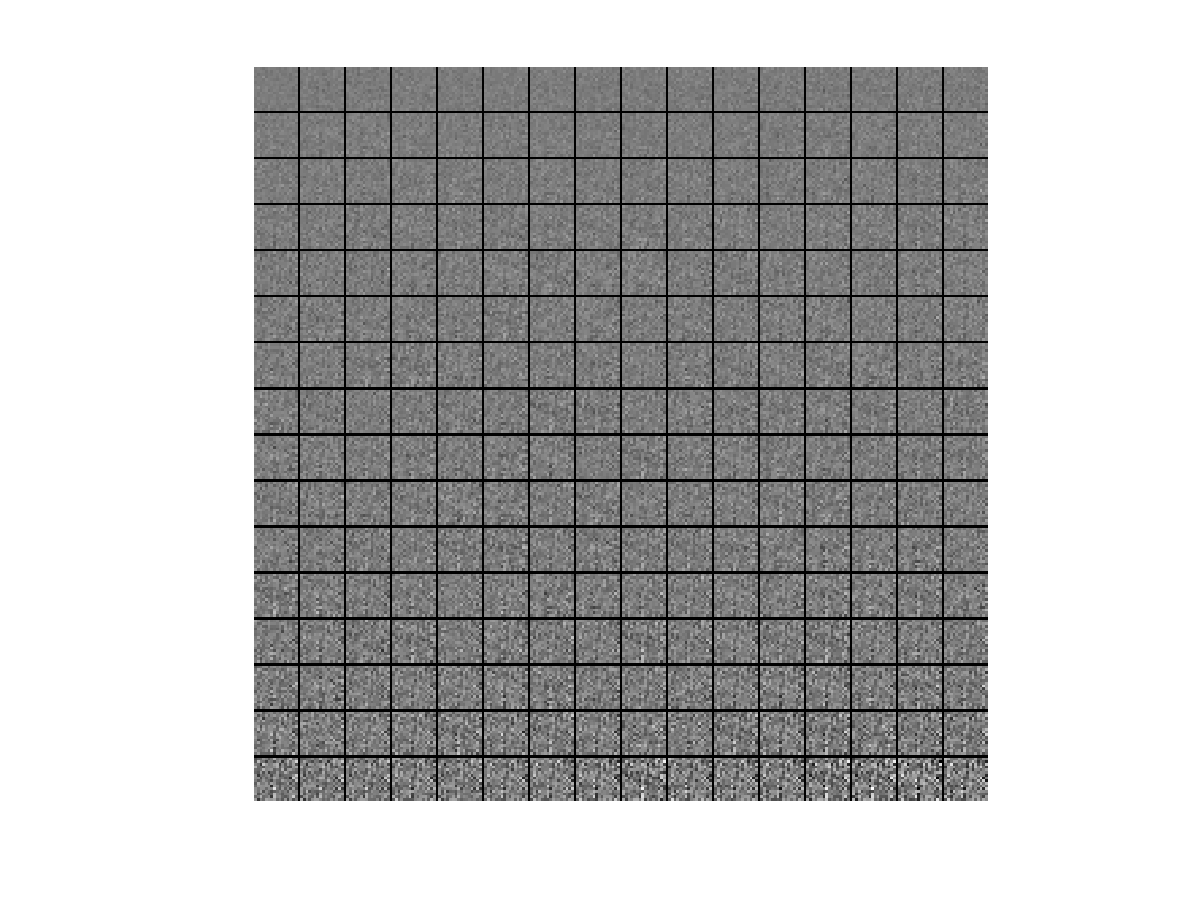
\includegraphics[width=\textwidth]{q3/ica_filters.png}
        \caption{ICA unmixing matrix}
        \label{fig:ica}
    \end{subfigure}
    ~ %add desired spacing between images, e. g. ~, \quad, \qquad, \hfill etc. 
      %(or a blank line to force the subfigure onto a new line)
    \begin{subfigure}[b]{0.4\textwidth}
        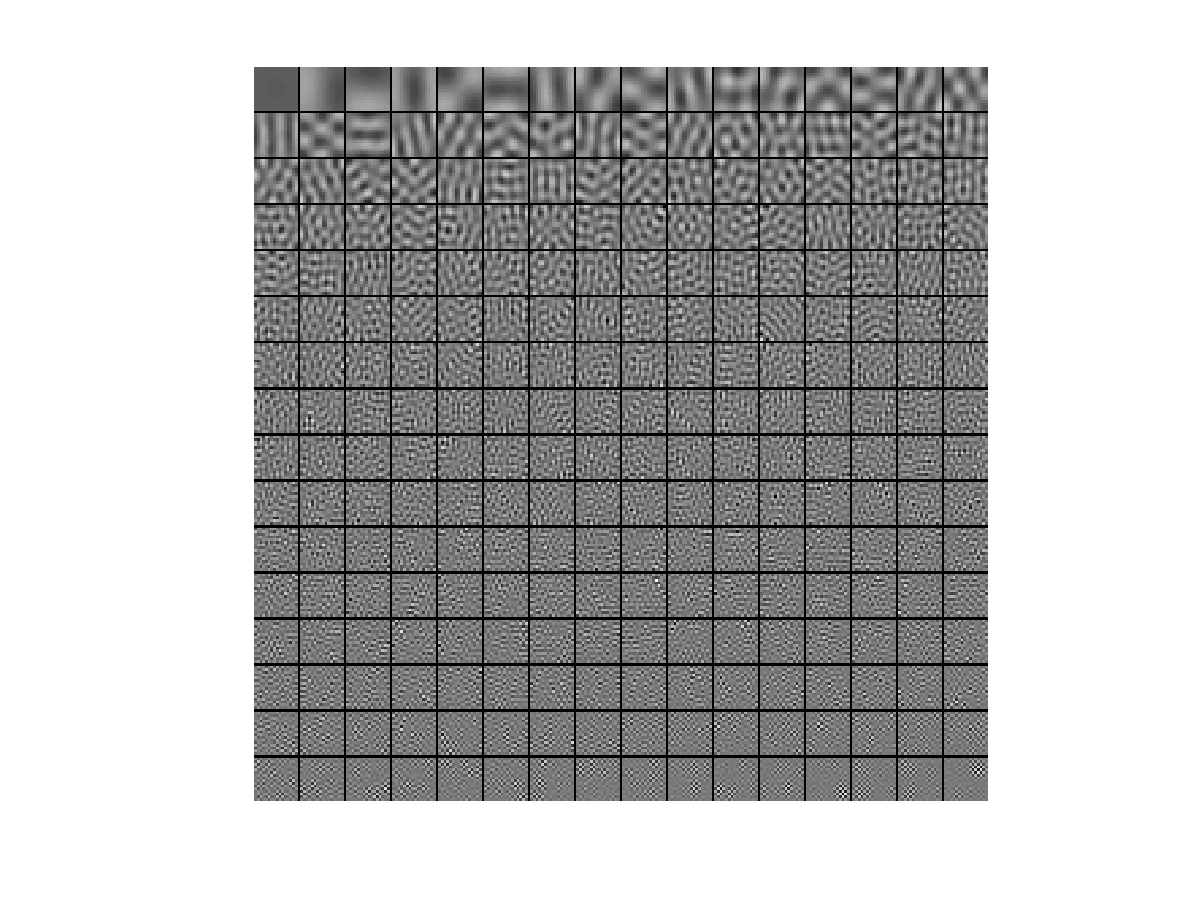
\includegraphics[width=\textwidth]{q3/pca_filters.png}
        \caption{PCA principal components matrix}
        \label{fig:pca}
    \end{subfigure}
\end{figure}

The ICA unmixing matrix separates the input data into its original sources, while the PCA principal components matrix represents the principal dimensions the data lies in.

\section*{4}
\subsection*{a)}
Let $s \in \mathbb{S}$ be any state in $\mathbb{S}$.\\
Let $s' \sim P_{s \pi(s)}$ be a random variable drawn from the $P_{s \pi(s)}$ distribution.\\
Since $V_1(s) \le V_2(s) \quad \forall s \in \mathbb{S}$,\quad$V_1(s') \le V_2(s')$, and we have
\begin{align*}
    V_1(s') &\le V_2(s') \\
    E_{s' \sim P_{s \pi(s)}}[V_1(s')] &\le E_{s' \sim P_{s \pi(s)}}[V_2(s')] \\
    \gamma E_{s' \sim P_{s \pi(s)}}[V_1(s')] &\le \gamma E_{s' \sim P_{s \pi(s)}}[V_2(s')] \\
    R(s) + \gamma E_{s' \sim P_{s \pi(s)}}[V_1(s')] &\le R(s) + \gamma E_{s' \sim P_{s \pi(s)}}[V_2(s')] \\
    B(V_1)(s) &\le B(V_2)(s) \quad \forall s \in \mathbb{S} \\
\end{align*}

\subsection*{b)}
\begin{align*}
    ||B^{\pi}(v) - V^{\pi}||_{\infty} &= ||R(s) + \gamma \sums P_{s \pi(s)}(s') V(s') - (R(s) + \gamma \sums P_{s \pi(s)}(s') V^{\pi}(s')) ||_{\infty} \\
                                    &= ||\gamma \sums P_{s \pi(s)}(s') V(s') - P_{s \pi(s)}(s') V^{\pi}(s') ||_{\infty} \\
                                    &= ||\gamma \sums P_{s \pi(s)}(s') (V(s') - V^{\pi}(s')) ||_{\infty} \\
                                    &= \max_{s' \in \mathbb{S}} \big[ \gamma \sums P_{s \pi(s)}(s') (V(s') - V^{\pi}(s')) \big] \\
                                    &= \gamma \max_{s' \in \mathbb{S}} \big[ \sums P_{s \pi(s)}(s') (V(s') - V^{\pi}(s')) \big] \\
                                    &= \gamma \max_{s' \in \mathbb{S}} \big[ E_{s' \sim P_{s \pi(s)}}[V(s') - V^{\pi}(s')] \big] \\
                                    &\le \gamma \max_{s' \in \mathbb{S}} \big[ \max_{s' \in \mathbb{S}}[V(s') - V^{\pi}(s')] \big] \\
                                    &= \gamma \max_{s' \in \mathbb{S}} \big[ V(s') - V^{\pi}(s') \big] \\
                                    &= \gamma || V - V^{\pi} ||_{\infty} \\
\end{align*}
Therefore $||B^{\pi}(v) - V^{\pi}||_{\infty} \le \gamma || V - V^{\pi} ||_{\infty}$. \\

\section*{5}

See q5/ folder for code.

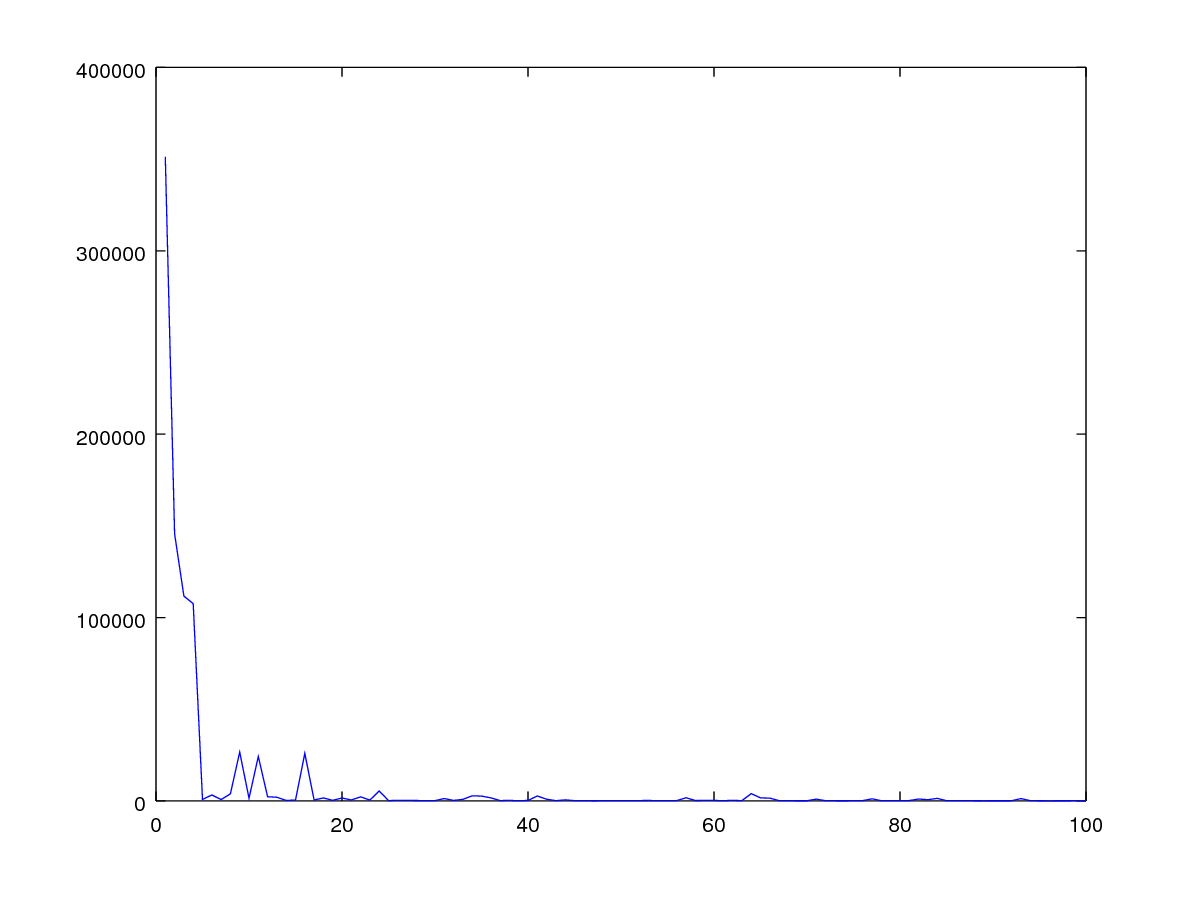
\includegraphics[width=0.5\textwidth]{q5/learning_curves.png}

x-axis is episode number, y-axis is number of steps before the car reached the top of the hill. The values plotted represent an average over 20 runs (i.e. there were 20 runs where each run contains 100 episodes).

\end{document}

